% Text for chapter 1
\chapter{Introduction}\label{ch:introduction}

% Figure manager for Chapter 1
% spell-checker: disable
\begin{pycode}[chapter1]
name = 'chapter1'
ch1 = texfigure.Manager(
    pytex,
    os.path.join('.', name),
    number=1,
    **{k: os.path.join('.', name, v) for k,v in manager_opts.items()}
)
from matplotlib.path import Path
import matplotlib.patches

from formatting import remove_ticks_and_spines
\end{pycode}
% spell-checker: enable

Perhaps no other consistent celestial event has attracted as much attention as the total solar eclipse. Solar eclipses have been observed and recorded for thousands of years, with some reports dating back to the fourteenth century BC \citep{golub_solar_2010}. The recordings of ancient eclipses have been heavily studied. Chinese rock drawings dating back to the Han dynasty (approximately 1900 years ago) appear to show the moon completely obscuring the Sun. Most recently on 21 August 2017, the ``Great American Eclipse'' captured the attention of millions from Oregon to South Carolina as it diagonally traversed the United States, offering a breathtaking view of the otherwise-invisible solar corona. 

The Sun is the most important celestial body to life on Earth. For the last five billion years, it has provided the light by which humans observe the world around them and the heat to save the planet from the frigid temperatures of interplanetary space. Because of its proximity, the Sun provides astronomers an exclusive and unique look into how stars behave. At the same time, space weather on Earth driven by magnetized material ejected from the solar atmosphere, threatens modern technological infrastructure.

The focus of this thesis is the solar corona, the outermost layer of the Sun's atmosphere and the manner in which energy is deposited into the hot, tenuous coronal plasma. This chapter serves as a brief introduction to the astrophysics of the Sun and its dynamic and highly-complex atmosphere. In \autoref{sec:structure}, I give a brief description of the interior of the Sun and the layers of the solar atmosphere. \autoref{sec:magnetic-field} describes the magnetic field of the Sun and \autoref{sec:coronal-heating} introduces the coronal heating problem.

\section{The Structure of the Solar Atmosphere}\label{sec:structure}

The Sun is a main-sequence G2 type star and its current age is $\approx\SI{4.6e9}{\year}$. It has a mass of $M_\solar = \SI{1.99e33}{\gram}$ and a radius of $R_\solar = \SI{6.955e10}{\cm}$ \citep{priest_magnetohydrodynamics_2014}. The Sun emits primarily as a blackbody in the visible and the infrared and the effective temperature of the surface is $T_\textup{eff}=\SI{5777}{\kelvin}$ \citep{carroll_introduction_2007}. However, as will be discussed in later sections, the temperature structure of the solar atmosphere is far more complicated. In the following sections, I discuss the structure of the stellar interior (\autoref{sec:interior}) and then give a brief description of each layer of the solar atmosphere: the photosphere (\autoref{sec:photosphere}), the chromosphere (\autoref{sec:chromosphere}), the transition region (\autoref{sec:transition_region}), and finally the corona (\autoref{sec:corona}).

\subsection{Interior}\label{sec:interior}

% spell-checker: disable %
\begin{pycode}[chapter1]
from matplotlib.patches import Wedge
# set location parameters
xcen,ycen = -0.5,0
theta = 33
ctheta = np.cos(theta * np.pi/180)
stheta = np.sin(theta * np.pi/180)

# setup figure and axes
fig = plt.figure(figsize=texfigure.figsize(
    pytex,
    scale=1,
    height_ratio=0.8,
))
ax = fig.gca()
ax.set_ylim(-0.75,0.75)
ax.set_xlim(-0.75,0.75)
ax.set_aspect('equal')
remove_ticks_and_spines(ax)

# Core
w_c = Wedge((xcen,ycen), 0.3, -theta, theta,
            facecolor=PALETTE[3], edgecolor='k')
ax.add_patch(w_c)
ax.text(0.3*ctheta+xcen, 0.3*stheta+ycen, r'$0.3R_\odot$',
        verticalalignment='bottom', horizontalalignment='center',
        rotation=theta)
ax.annotate('Core',
            xy=(xcen + 0.3/2, ycen), xycoords='data',
            xytext=(xcen-0.1,-0.35+ycen), textcoords='data',
            arrowprops=dict(
                arrowstyle="-|>",
                color='k',
                shrinkA=15, shrinkB=0,
                patchA=None,
                patchB=None,
                connectionstyle='angle,angleA=180,angleB=-90,rad=0',
            ),
)

# Radiative zone
w_r = Wedge((xcen,ycen), 0.714, -theta, theta,
            width=0.714-0.3,
            facecolor=PALETTE[1], edgecolor='k')
ax.add_patch(w_r)
ax.text(0.714*ctheta+xcen, 0.714*stheta+ycen,
        r'$0.714R_\odot$',
        verticalalignment='bottom', horizontalalignment='center',
        rotation=theta)
ax.annotate('Radiative Zone',
            xy=(xcen + 0.25 + (0.714-0.3)/2, ycen),xycoords='data',
            xytext=(xcen-0.2,ycen+0.4),textcoords='data',
            arrowprops=dict(
                arrowstyle="-|>",
                color='k',
                shrinkA=50, shrinkB=0,
                patchA=None,
                patchB=None,
                connectionstyle='angle,angleA=180,angleB=-90,rad=0',
            ),
)

# Convection zone
w_con = Wedge((xcen,ycen), 1, -theta, theta,
              width=1-0.714,
              facecolor=PALETTE[0], edgecolor='k')
ax.add_patch(w_con)
ax.text(1*ctheta+xcen, 1*stheta+ycen,
        r'$1R_\odot$',
        verticalalignment='bottom', horizontalalignment='center',
        rotation=theta)
ax.annotate('Convection Zone',
            xy=(xcen + 0.714 + (1-0.714)/2, ycen),xycoords='data',
            xytext=(xcen+1,ycen+0.4),textcoords='data',
            arrowprops=dict(
                arrowstyle="-|>",
                color='k',
                shrinkA=10, #shrinkB=25,
                patchA=None,
                patchB=None,
                connectionstyle='angle,angleA=-90,angleB=180,rad=0',
            ),
)

#save
tfig = ch1.save_figure('interior-cartoon', fext='.pgf')
tfig.caption = r'Schematic of the solar interior. In the core and radiative zone, radiation is the dominant energy transfer mechanism while convection, the cyclic rise of hot gas to the surface and subsequent infall of cooled gas, dominates in the convection zone. Adapted from Figure 11.2 of \citet{carroll_introduction_2007}.'
\end{pycode}
\py[chapter1]|tfig|
% spell-checker: enable %

The interior of the Sun cannot be directly observed because it is opaque to radiation such that all knowledge of its structure must be inferred from detailed stellar structure calculations or through helioseismology, the study of global oscillations \citep{priest_magnetohydrodynamics_2014}. The solar interior can be divided into three distinct layers: the core, the radiative zone, and the convection zone. This is illustrated in \autoref{fig:interior-cartoon}.

\begin{figure}
    \tikzstyle{arrow} = [thick, ->, >=stealth]
    \tikzstyle{ghost} = [rectangle, rounded corners, text centered, draw=white]
    \centering
    \begin{tikzpicture}[node distance=2.5cm]
        % Create nodes
        \node(top){
            $\begin{aligned}
            \isotope[1][1]{H} + \isotope[1][1]{H} \to& \isotope[2][1]{H} + e^+ + \nu_e \\
            \isotope[2][1]{H} + \isotope[1][1]{H} \to& \isotope[3][2]{H} + \gamma
            \end{aligned}$
        };
        \node(g1)[below of=top]{};
        \node(pp1)[left of=g1]{
            $\begin{aligned}
            \isotope[3][2]{He} + \isotope[3][2]{He} \to& \isotope[4][2]{He} + 2\isotope[1][1]{H} \\
            (\textup{ppI})&
            \end{aligned}$
        };
        \node(pp23)[right of=g1]{
            $\isotope[3][2]{He} + \isotope[4][2]{He} \to \isotope[7][4]{Be} + \gamma$
        };
        \node(g2)[below of=pp23]{};
        \node(pp2)[left of=g2]{
            $\begin{aligned}
            \isotope[7][4]{Be} + e^- \to& \isotope[7][3]{Li} + \nu_e \\
            \isotope[7][3]{Li} + \isotope[1][1]{H} \to& 2\isotope[4][2]{He} \\
            (\textup{ppII})&
            \end{aligned}$
        };
        \node(pp3)[right of=g2]{
            $\begin{aligned}
            \isotope[7][4]{Be} + \isotope[1][1]{H} \to& \isotope[8][5]{B} + \gamma \\
            \isotope[8][5]{B} \to& \isotope[8][4]{Be} + e^+ + \nu_e \\
            \isotope[8][4]{Be} \to& \isotope[4][2]{He} \\
            (\textup{ppIII})&
            \end{aligned}$
        };
        % Draw arrows
        \draw [arrow] (top) -- (pp1);
        \draw [arrow] (top) -- (pp23);
        \draw [arrow] (pp23) -- (pp2);
        \draw [arrow] (pp23) -- (pp3);
    \end{tikzpicture}
    \caption{The three branches of the proton-proton nucleosynthesis reaction. The ppI branching ratio is 69\% and the ppII branching ratio is 99.7\%. Adapted from Figure 10.8 in \citet{carroll_introduction_2007}.}
    \label{fig:pp-chain}
\end{figure}

The \textit{core} of the Sun is very hot, $\approx\SI{1.57e7}{\kelvin}$, and dense, $\approx\SI{9e25}{\per\cubic\cm}$ \citep{carroll_introduction_2007,bahcall_solar_2001} and, as denoted in \autoref{fig:interior-cartoon}, extends radially to $r\lesssim 0.3R_\solar$. The primary mechanism of energy production in the core is the fusion of \isotope[1][1]{H} into \isotope[4][2]{He} via a reaction called the proton-proton chains or the ``pp'' chains. Besides \isotope[4][2]{He}, the pp chain also produces positrons ($e^+$), weakly-interacting neutrinos ($\nu_e$) which travel uninhibited out of the interior, and photons ($\gamma$). The full reaction chain is shown in \autoref{fig:pp-chain}. These reactions can only occur at very high densities such as those found in the core as quantum tunneling is required to overcome the Coulomb barrier between the two \isotope[1][1]{H} atoms.

Moving radially outward from the core, the density drops, inhibiting the production of photons through the pp chain, and the temperature decreases such that $dT/dr < 0$. This decrease in temperature causes a decrease in radiation pressure with increasing $r$, leading to the slow upward diffusion of photons produced by the pp chain reactions. These photons thus undergo a ``random walk'' from the core to the surface as the photons are continually absorbed and reemitted isotropically. Radiation is the dominant energy transport mechanism in the region $0.3R_\solar\le r\le 0.714R_\solar$, often referred to as the radiative zone \citep{carroll_introduction_2007}. 

While radiation is the dominant transport process deep in the core, convection is  more efficient in the region $0.714R_\solar<r\le1R_\solar$, the so-called convective zone (see \autoref{fig:interior-cartoon}). As the temperature gradient continues to steepen, the opacity increases thus inhibiting energy transport by radiation and convection becomes the dominant transport mechanism. In particular, the transition from radiative to convective transport occurs when the temperature gradient becomes ``super adiabatic'' \citep[see Section 10.4 of][]{carroll_introduction_2007}. In the convective zone, hot, buoyant mass elements carry excess energy outward while cool mass elements fall inward and the cycle repeats, repeatedly carrying energy to the surface. 

\subsection{Photosphere}\label{sec:photosphere}

% spell-checker: disable %
\begin{pycode}[chapter1]
# Read in VAL atmosphere and interpolate
from hs_atmosphere import read_VAL3c_MTW, interpolate_atmosphere
data = read_VAL3c_MTW(
    ch1.data_file('VALIIIC.dat'),
    MTW_file=ch1.data_file('mcwhirter.dat')
)
Z = data['Z'].to(u.Mm)
atmos = interpolate_atmosphere(data, Z)

# Setup figure
fig = plt.figure(figsize=texfigure.figsize(
    pytex,
))
ax = fig.gca()
ax2 = ax.twinx()

# Plot
ax.plot(Z, data['T'].to(u.K), color=PALETTE[0], marker='o', ls='', markevery=2)
line_T = ax.plot(Z, atmos['T'].to(u.K), color=PALETTE[0], ls='-', label=r'$T$')
ax2.plot(Z, (data['p']/const.k_B/2/data['T']).to('cm^-3'),
            color=PALETTE[1], marker='o', ls='', markevery=2)
line_n = ax2.plot(Z, (atmos['p']/const.k_B/2/atmos['T']).to('cm^-3'),
                    color=PALETTE[1], ls='-', label=r'$n$')

# Labels
ax.set_xlabel(r'$h$ $[\si{\mega\m}]$')
ax.set_ylabel(r'$T$ $[\si{\kelvin}]$')
ax2.set_ylabel(r'$n$ $[\si{\per\cubic\cm}]$')
ax.set_xlim(Z[0].value,(5*u.Mm).value)
ax2.set_xlim(Z[0].value,(5*u.Mm).value)
ax.set_ylim(2e3,1e6)
ax.set_yscale('log')
ax2.set_yscale('log')

# Legend
lns = line_T + line_n
labs = [l.get_label() for l in lns]
ax.legend(lns, labs, frameon=False, loc='center right')

# Annotate regions
ax.vlines([Z[np.argmin(data['T'])].value, 2.15, 2.35], 2e3, 1e6,
            colors='k',linestyles='dotted',)
ax.annotate('Photosphere',
            xytext=(0.25,1.1), textcoords=('data','axes fraction'),
            xy=(0.25,0.7), xycoords=('data','axes fraction'),
            va='center',ha='center',
            arrowprops=dict(arrowstyle="-|>", color='k'),
)
ax.annotate('Chromosphere',
            xy=(1.25,3e5),xycoords='data',
            va='center',ha='center',
)
ax.annotate('Transition Region',
            xytext=(2.25,1.1), textcoords=('data','axes fraction'),
            xy=(2.25,0.7), xycoords=('data','axes fraction'),
            va='center',ha='center',
            arrowprops=dict(arrowstyle="-|>", color='k'),
)
ax.annotate('Corona',
            xy=(3.5,1e5),xycoords='data',
            va='center',ha='center',
)

# Save
tfig = ch1.save_figure('val-atmosphere', fext='.pgf')
tfig.caption = r'Temperature (blue, left axis) and density (orange, right axis) of the solar atmosphere as a function of height, $h$, above the solar surface. These profiles are based on the semi-empirical models of \citet{mcwhirter_heating_1975} and \citet{vernazza_structure_1981}. The data points show the exact values from the models and the smooth lines are first-order spline fits to the data. The dotted black lines denote the different regions of the solar atmosphere.'
\end{pycode}
\py[chapter1]|tfig|
% spell-checker: enable %

Just above the convection zone lies the \textit{photosphere}, the lowest layer of the solar atmosphere and often considered the ``surface'' of the Sun. The photosphere is a dense, relatively thin layer and can be observed in visible light. Here, the optical depth, $\tau$, or the transparency of the plasma, is $\tau\lesssim1$ in the visible band such that photons in these wavelengths can escape without being absorbed and reemitted. Thus, most of the Sun's emission in the visible spectrum originates in the photosphere \citep{priest_magnetohydrodynamics_2014}. The photosphere extends to approximately $\SI{500}{\km}$ above the surface and corresponds to a minimum in the temperature as a function of height, $T_\textup{min}\approx\SI{4400}{\kelvin}$. This is illustrated in \autoref{fig:val-atmosphere}. The definition of the base of the photosphere is a bit more arbitrary, but is usually said to be $\approx\SI{100}{\km}$ below the point where $\tau\sim1$ for photons of wavelength \SI{5e3}{\angstrom} \citep{carroll_introduction_2007}. 

The top left panel of \autoref{fig:example-images} shows an observation of the photosphere at \SI{4500}{\angstrom} by the Atmospheric Imaging Assembly instrument \citep[AIA][]{lemen_atmospheric_2012} on the Solar Dynamics Observatory spacecraft \citep[SDO][]{pesnell_solar_2012}. Note that the image appears relatively smooth as the Sun emits primarily as a blackbody in the visible and infrared wavelengths \citep{carroll_introduction_2007}.

\subsection{Chromosphere}\label{sec:chromosphere}

Above the photosphere lies the \textit{chromosphere} which has a depth of $\approx\SI{1600}{\km}$. Moving upward through the chromosphere from the temperature minimum at the top of the photosphere, the temperature increases at first gradually and then more rapidly with increasing height to many times \SI{e4}{\kelvin} (see \autoref{fig:val-atmosphere}). At the same time, the density is falling off very rapidly. Though not visible with the naked eye, the chromosphere is highly structured. Spicules, tall columns of gas that extend high into the solar atmosphere thought to heavily impact the behavior of plasma in the corona \citep{de_pontieu_origins_2011}, are primarily visible off the solar disk in $\isotope{H}\alpha$ and originate in the photosphere in addition to filaments (spicules observed on-disk) and plage, bright regions surrounding sunspots.

% spell-checker: disable %
\begin{pycode}[chapter1]
# Import all maps
maps = []
names = [
    'aia_4500_example',
    'aia_304_example',
    'aia_171_example',
    'xrt_example'
]
for i in names:
    maps.append(Map(ch1.data_file(f'{i}.fits' )))
# Fix XRT metadata
maps[3] = Map(
    maps[3].data,
    {**maps[3].meta, 'wavelnth': f'{maps[3].meta["ec_fw1_"]}/{maps[3].meta["ec_fw2_"]}'}
)
# Set colormap normalization
for i,m in enumerate(maps):
    f = 1 if i == 0 else 0.1
    m.plot_settings['norm'] = ImageNormalize(vmin=max(0,m.data.min()),
                                             vmax=f*m.data.max(),
                                             stretch=AsinhStretch(0.1))

# Make figure
fig = plt.figure(figsize=texfigure.figsize(
    pytex,
    scale=1,
    height_ratio=1,
))
for i,m in enumerate(maps):
    ax = fig.add_subplot(2, 2, i+1, projection=m)
    m.plot(axes=ax,annotate=False,)
    ax.grid(alpha=0)
    lon,lat = ax.coords[0],ax.coords[1]
    lon.set_ticks_visible(False)
    lon.set_ticklabel_visible(False)
    lat.set_ticks_visible(False)
    lat.set_ticklabel_visible(False)
    lon.frame.set_linewidth(0)
    lat.frame.set_linewidth(0)
    try:
        wvl = m.meta['wavelnth'] * u.Angstrom
        wvl = f"{m.meta['wavelnth']} {u.Angstrom.to_string(format='latex')}"
    except ValueError:
        wvl = m.meta['wavelnth']
    ax.text(20, m.dimensions.y.value-20,
            f'{m.observatory}/{m.instrument.split(" ")[0]} {wvl}',
            color='w',
            fontsize=plt.rcParams['legend.fontsize']*0.75,
            horizontalalignment='left',
            verticalalignment='top',)
    ax.text(m.dimensions.x.value-20,20,
            astropy.time.Time(m.date).strftime('%Y/%d/%m'),
            color='w',
            fontsize=plt.rcParams['legend.fontsize']*0.75,
            horizontalalignment='right',
            verticalalignment='bottom')
plt.subplots_adjust(hspace=0.01,wspace=0.01)

# Save figure
tfig = ch1.save_figure('example-images', fext='.pdf')
tfig.caption = r"The layers of the Sun's atmosphere Sun as revealed by multiple wavelengths at approximately 19:00 UTC on 2010 December 1. The top left panel shows the photosphere, the top right panel shows chromosphere, and the bottom left panel shows the EUV corona all imaged by SDO/AIA. The bottom right panel shows the hot X-ray corona as observed by \textit{Hinode}/XRT. All data are courtesy of the AIA and XRT instrument teams."
tfig.placement = '!h'
\end{pycode}
\py[chapter1]|tfig|
% spell-checker: enable %

The top right panel \autoref{fig:example-images} shows the chromosphere as observed by the \SI{304}{\angstrom} channel of SDO/AIA. Note that the chromosphere is much more highly structured compared to the underlying photosphere.

\subsection{Transition Region}\label{sec:transition_region}

The extremely thin \textit{transition region} (TR) sits between the chromosphere and the corona and primarily emits emission in the extreme ultraviolet (EUV) portion of the electromagnetic spectrum. It is only a few hundred \si{\km} thick, but is characterized by very steep temperature gradients as the temperature increases over an order of magnitude, from a few \SI{e4}{\kelvin} to well above \SI{e5}{\kelvin}, as illustrated in \autoref{fig:val-atmosphere}. The density also continues to rapidly decrease in the TR.

The upper boundary of the TR is not static and is more properly defined in terms of the role of thermal conduction in the TR energy balance. This is discussed in more detail in \autoref{sec:heat-flux}.  

\subsection{Corona}\label{sec:corona}

The outermost layer of the solar atmosphere is the \textit{corona} (Latin, ``crown'') and begins a little over \SI{2e3}{\km} above the surface. The corona is very hot ($\gtrsim\SI{e6}{\kelvin}$) and diffuse ($\lesssim\SI{e9}{\per\cubic\cm}$) and is characterized primarily by \textit{optically-thin} emission in the X-ray and EUV bands such that photons are not reemitted or absorbed once they are produced in the corona. The corona is only visible by the naked eye during an eclipse.

The corona is highly-structured by the complex coronal magnetic field into \textit{coronal loops} because of the relative strength of the magnetic field compared to the gas pressure (see \autoref{ch:loops}). These hot, dynamic structures emit primarily in the EUV and X-ray. The bottom panels of \autoref{fig:example-images} show the corona at $\approx\SI{8e5}{\kelvin}$ as imaged by the \SI{171}{\angstrom} channel of SDO/AIA (left panel) and at $\approx\SI{e7}{\kelvin}$ as imaged by the X-ray Telescope \citep[XRT][]{golub_x-ray_2007} on the \textit{Hinode} satellite \citep{kosugi_hinode_2007}. Note how drastically the appearance of the Sun changes moving upward from the photosphere (top left) to the chromosphere (top right) to the EUV corona (bottom left). The dynamics of these EUV- and X-ray-bright loop structures in the corona is the primary focus of this thesis.

Above the corona, the solar atmosphere transitions to empty space. If the solar magnetic field is open such that it connects to the interplanetary magnetic field rather than closing back at the surface, particles can escape from the Sun into the \textit{solar wind}. The existence of the solar wind was first predicted by \citet{parker_dynamics_1958} based on the relatively simple idea that a hot, hydrostatic corona should be expanding given the pressure measured in interplanetary space. The solar wind has two components: a fast solar wind with velocity $\approx\SI{800}{\km\per\second}$ and a slow solar wind with velocity $\approx\SI{400}{\km\per\second}$ \citep{golub_solar_2010}. While it is generally agreed that the fast wind originates from cool, dark coronal holes, the origin of the slow wind is much less certain.

\section{The Solar Magnetic Field}\label{sec:magnetic-field}

Like the Earth, the Sun possesses an intrinsic magnetic field. Near the polar regions, the solar magnetic field is approximately dipolar, but closer to the equator, the field is highly nonuniform and dynamic. In areas of intense magnetic activity, the magnetic field strength can reach a few \SI{e3}{\gauss}\footnote{For reference, the Earth's magnetic field at its surface has an average value of $\approx\SI{0.5}{\gauss}$ \citep{finlay_international_2010}.} while in more ``quiet'' regions, it is much lower, \SIrange{0.1}{0.5}{\gauss} \citep{aschwanden_physics_2006}. Interestingly, global magnetic activity on the Sun varies on a $\approx\SI{11}{\year}$ cycle in which the dipolar also reverses \citep{golub_solar_2010}. The exact physical mechanism responsible for this cyclic variability and the generation of the intrinsic field are not well understood. 

The solar magnetic field extends high into the solar atmosphere and dominates the structuring and dynamics in the hot, tenous corona. Because of the high temperatures that characterize both the solar atmosphere and interior, much of the gas that makes up the Sun is ionized; that is, each atom has been stripped of at least one of its electrons. This means that the Sun is filled by a sea of charged particles called a \textit{plasma}. Because these particles are charged, the dynamics of the plasma are strongly influenced by solar magnetic field and vice versa such that the solar plasma and magnetic field represent a coupled system. In general, the coupled dynamics of the solar plasma and magnetic field are described by the equations of \textit{magnetohydrodynamics} (MHD),
\begin{align}
    &\frac{d}{dt}\rho + \rho\nabla\cdot\mathbf{v} = 0, \label{eq:mhd_continuity} \\
    &\rho\frac{d}{dt}\mathbf{v} = \frac{1}{c}\mathbf{j}\times\mathbf{B} - \nabla p, \label{eq:mhd_momentum} \\
    &\mathbf{j} = \frac{c}{4\pi}\nabla\times\mathbf{B}, \label{eq:mhd_ampere} \\
    &\frac{\partial}{\partial t}\mathbf{B} = \nabla\times(\mathbf{v}\times\mathbf{B}) + \frac{\eta c^2}{4\pi}\nabla^2\mathbf{B}, \label{eq:mhd_faraday} \\
    &\nabla\cdot\mathbf{B} = 0, \label{eq:mhd_divb} \\
    &\frac{\rho^\gamma}{\gamma - 1}\frac{d}{dt}\left(\frac{p}{\rho^{\gamma}}\right) = -\nabla\cdot\mathbf{q} - R + H, \label{eq:mhd_energy}
\end{align}
where $\rho$ is the mass density, $\mathbf{v}$ is the bulk flow velocity, $\mathbf{j}$ is the current density, $\mathbf{B}$ is the magnetic field, $p$ is the thermal pressure, $\eta$ is the magnetic diffusivity, $\gamma=5/3$ is the ratio of specific heats, $\mathbf{q}$ is the heat flux, $R$ is the radiative loss term, $H$ is heating due to Ohmic and viscous dissipation, and $d/dt\equiv\partial/\partial t + \mathbf{v}\cdot\nabla$ \citep{priest_magnetohydrodynamics_2014}. Solving the MHD equations for the time-dependent, vector magnetic field in three-dimensions is an extremely challenging problem that requires sophisticated numerical codes and significant computational resources.

\subsection{Origin of the Magnetic Field and Flux Emergence}\label{sec:magnetic-origins}

The generation and emergence of the complex magnetic field at the surface is due primarily to two mechanisms in the solar interior: differential rotation and convection. Because the Sun is not a rigid body, the rotation rate of the solar plasma varies latitudinally as well as radially where the radial dependence is also latitude dependent. In particular, at a latitude of \SI{60}{\degree}, the solar interior seems to rotate faster than the surface while the opposite is true at the equator \citep{thompson_differential_1996}. At $r\sim0.6R_\solar$ near the base of the convection zone (see \autoref{fig:interior-cartoon}) the rotation rates at all latitudes converge \citep{golub_solar_2010}. This region of convergence is often called the tachocline \citep{aschwanden_physics_2006}.

This radial dependence of the rotation rate is important to the magnetic field because the field is magnetic field is ``frozen-in'' to the plasma. Another way of stating this is that the magnetic flux $\Phi=\int_\Sigma\dd{\mathbf{S}}\cdot\mathbf{B}$ through a surface $\Sigma$ does not change in time along the path of a fluid element such that,
\begin{equation}\label{eq:frozen-flux}
    \frac{d}{dt}\Phi = 0.
\end{equation}
As proof of this, consider a small change in flux $\delta\Phi$ as the fluid element travels through two surfaces $\Sigma$ and $\Sigma^\prime$ in time $\delta t$ with velocity $\mathbf{v}$. $\delta\Phi$ can be expressed as,
\begin{equation*}
    \delta\Phi = \int_{\Sigma^\prime}\dd{\mathbf{S}}\cdot\mathbf{B}(t+\delta t) - \int_\Sigma\dd{\mathbf{S}}\cdot\mathbf{B}(t).
\end{equation*}
Using the divergent-free condition of $\mathbf{B}$ (\autoref{eq:mhd_divb}) combined with Stoke's theorem and the fact that $\dd{\mathbf{S}}=\dd{\ell}\times\delta t\mathbf{v}$ gives,
\begin{align}
    \delta\Phi =& \int_\Sigma\dd{\mathbf{S}}\cdot(\mathbf{B}(t+\delta t) - \mathbf{B}(t)) - \delta t\oint_\mathcal{C}\dd{\ell}\cdot\mathbf{v}\times\mathbf{B}(t + \delta t), \nonumber\\
    \frac{\delta\Phi}{\delta t} =& \int_\Sigma\dd{\mathbf{S}}\cdot\left( \frac{\mathbf{B}(t+\delta t)}{\delta t} - \nabla\times(\mathbf{v}\times\mathbf{B}(t + \delta t)) \right),\nonumber
\end{align}
where $\mathcal{C}$ is the curve that encloses $\Sigma$. Taking the limit $\delta t\to0$ and using the ideal MHD induction equation (\autoref{eq:mhd_faraday} with $\eta=0$) gives \autoref{eq:frozen-flux}.

Under the condition of \autoref{eq:frozen-flux} the magnetized plasma drags the magnetic field with along with it. Following the treatment of \citet{golub_solar_2010}, an initially straight magnetic field line oriented along the solar rotation axis, the plasma frozen to the field line will undergo differential rotation such that the field line will be stretched perpendicular to the original orientation. As the Sun continues to rotate, the field is continually ``wound up'' and the perpendicular component increases. This amplification of effect of an initially dipolar field is purely a consequence of differential rotation and the assumption of flux freezing (\autoref{eq:frozen-flux}) and provides a qualitative picture for the generation of the intrinsic magnetic field of the Sun. A more quantitative approach requires solving the non-linear dynamo equations \citep[see Section 4.3.3 of][]{golub_solar_2010}.

As the magnetic field in the solar interior becomes continually deformed due to differential rotation, these twisted magnetic field lines are carried upward through the convection zone to the surface due to magnetic buoyancy. First proposed by \citet{parker_formation_1955}, this effect occurs when the internal pressure of plasma plus the magnetic pressure of the frozen-in field cannot balance the ambient pressure, thus forcing the field line upward. This twisted and amplified field is carried up through the photosphere, forming dipolar loop-like structures that extend high above the surface and into the chromosphere, transition region, and corona. This phenomenon, called flux emergence, leads to the formation of \textit{active regions}, areas of intense magnetic activity characterized by densely-packed closed magnetic structures.

Active regions are manifested as cool, dark sunspots in the photosphere due to the reduced internal pressure required to bring the flux to the surface. Additionally, the corona is typically referred to as a ``low-$\beta$'' plasma where,
\begin{equation}\label{eq:plasma-beta}
    \beta\equiv\frac{8\pi p}{B^2},
\end{equation}
is the ratio between the gas pressure ($p$) and the magnetic pressure ($B^2/8\pi$) and $\beta\ll1$ in an active region. As a result, active regions appear as bright loop-like structures in the EUV and X-ray bands as plasma is heated to temperatures in excess of several million \si{\kelvin} and traces out the magnetic field. The multi-wavelength appearance of an \AR{} can be seen in the top right quadrants of the top left (photosphere) and bottom (EUV and X-ray) panels in \autoref{fig:example-images}.

\subsection{Observations}\label{sec:magnetic-observations}

Knowledge of the magnetic field in the corona is crucial to understanding the dynamics and heating (see \autoref{sec:coronal-heating}) of the coronal plasma. However, direct measurements of the coronal vector magnetic field have proved challenging\footnote{The Daniel K. Inouye Telescope \citep{elmore_daniel_2014}, with expected first light in 2020, is expected to provide vastly improved measurements of the coronal magnetic field via high-resolution spectropolarimetry.} because the optical and infrared coronal lines sensitive to the field are relatively faint compared to the much brighter solar disk \citep{judge_coronal_2001}. As such, it is common practice to measure the LOS component of the photospheric magnetic field and then treat this measurement as a lower boundary condition for a model of the coronal field (see \autoref{sec:field_extrapolation}). The photospheric field can be measured using the \textit{Zeeman effect} wherein the magnetic field ``breaks'' the degeneracy of the atomic energy levels with respect to the total angular momentum operator. The resulting level splitting can be approximated by,
\begin{equation}\label{eq:zeeman}
    \Delta\lambda \approx 5\times10^{-13}B\lambda_0^2,
\end{equation}
where $B$ is the field strength and $\lambda_0$ is the wavelength when $B=0$ \citep{phillips_ultraviolet_2008}. In order for this splitting to be resolved compared to the instrument or thermal width, $B$ must be sufficiently strong and $\lambda_0$ sufficently long such that measurements of the coronal field ($B\sim\SI{e3}{\gauss}$) can only be made in the infrared.

% spell-checker: disable %
\begin{pycode}[chapter1]
# Prepare map
m = Map(ch1.data_file('hmi_example.fits')).rotate(order=3)
x, y = np.meshgrid(*[np.arange(v.value) for v in m.dimensions]) * u.pixel
hpc_coords = m.pixel_to_world(x, y)
r = np.sqrt(hpc_coords.Tx ** 2 + hpc_coords.Ty ** 2) / m.rsun_obs
mask = np.ma.masked_greater(r, 1)
m = Map(m.data, m.meta, mask=mask.mask)

# Build figure
scale = 0.45
fig = plt.figure(figsize=texfigure.figsize(
    pytex,
    scale=scale,
    height_ratio=1,
    figure_width_context='figurewidth',
))
ax = fig.gca(projection=m)
im = m.plot(
    axes=ax,
    annotate=False,
    title=False,
    cmap='better_RdBu_r',
    norm=matplotlib.colors.SymLogNorm(10, vmin=-7.5e2, vmax=7.5e2)
)

# Remove frame, HPC grid, add HGS grid
ax.grid(alpha=0)
lon,lat = ax.coords[0], ax.coords[1]
lon.frame.set_linewidth(0)
lat.frame.set_linewidth(0)
lon.set_ticks_visible(False)
lat.set_ticks_visible(False)
lon.set_ticklabel_visible(False)
lat.set_ticklabel_visible(False)
m.draw_grid(axes=ax, color='k', alpha=0.25, lw=0.5, grid_spacing=30*u.deg)

# Save
tfig = ch1.save_figure('example-magnetogram', fext='.pdf')
tfig.caption = r'The LOS magnetic field strength at the photosphere (i.e. a magnetogram) as measured by the HMI instrument on the SDO spacecraft at 19:00 UTC 2010 December 1. Red indicates positive polarity (out of the page) and blue indicates negative polarity (into the page). The colorbar is on a semi-log scale from $-\SI{750}{\gauss}$ to $+\SI{750}{\gauss}$.'
tfig.figure_width = r'{}\textwidth'.format(scale)
\end{pycode}
\py[chapter1]|tfig|
% spell-checker: enable %

Many ground-based telescopes \citep[e.g. GONG, Mt. Wilson][]{howard_mount_1976} and space-based instruments \citep[e.g. SOHO/MDI][]{scherrer_solar_1995} provide high-quality measurements of the LOS photospheric magnetic field. \autoref{fig:example-magnetogram} shows a full-disk magnetogram produced from measurements by the Helioseismic Magnetic Imager \citep[HMI,][]{hoeksema_helioseismic_2014} on SDO which measures the Fe I \SI{6173.34}{\angstrom} absorption line. Note that the region of enhanced adjacent positive and negative polarities seen in the top right quadrant is spatially coincedent with the sunspot and bright loops seen in the photospheric, EUV, and X-ray images in \autoref{fig:example-images}.

\subsection{Field Extrapolation}\label{sec:field_extrapolation}

\textit{Magnetic field extrapolation} is a commonly-used technique for approximating the three-dimensional vector magnetic field in the corona from a line-of-sight (LOS) measurement of the photospheric field strength. Following the treatment in \citet[Chapter 3]{priest_magnetohydrodynamics_2014}, \autoref{eq:mhd_momentum}, the ideal MHD momentum equation, in magnetohydrostatic balance can be written as,
\begin{equation}\label{eq:magnetohydrostatic_balance}
    0 = \frac{1}{c}\mathbf{j}\times\mathbf{B} - \nabla p.
\end{equation}
In a low-$\beta$ plasma (see \autoref{eq:plasma-beta}), the first term on the right-hand side can often be neglected such that \autoref{eq:magnetohydrostatic_balance} becomes,
\begin{equation}\label{eq:force_free}
    \mathbf{j}\times\mathbf{B} = 0.
\end{equation}
\autoref{eq:force_free} is the so-called \textit{force-free} condition. Combined with \autoref{eq:mhd_ampere}, Amp\'{e}re's law, this implies that,
\begin{equation}\label{eq:ampere_force_free}
    \nabla\times\mathbf{B} = \alpha\mathbf{B},
\end{equation}
where, in general, the scalar $\alpha$ may be some function of position $\mathbf{r}$.

In the case of $\alpha=0$, $\mathbf{j}=0$ (from \autoref{eq:mhd_ampere}) and the magnetic field is said to be current-free or \textit{potential}. \autoref{eq:ampere_force_free} implies that $\mathbf{B}$ is also curl-free such that it can be expressed as,
\begin{equation}\label{eq:b_potential}
    \mathbf{B}=\nabla\phi,
\end{equation}
 where $\phi$ is some scalar potential. Combining this expression with the requirement from Maxwell's equations that the magnetic field must always be divergence-free (\autoref{eq:mhd_divb}) gives Laplace's equation,
\begin{equation}\label{eq:laplace}
    \nabla^2\phi = 0.
\end{equation}
If the normal component of the magnetic field is specified on the lower boundary (e.g. from a photospheric LOS magnetogram), the solution within a closed volume is unique \citep{priest_magnetohydrodynamics_2014}.

Several methods have been developed to solve \autoref{eq:laplace} for the coronal magnetic field. The potential field source surface (PFSS) model of \citet{schatten_model_1969} solves \autoref{eq:laplace} for the global corona given a synoptic photospheric magnetogram as the lower boundary input and under the assumption that the field is purely radial at some ``source surface'', typically $2.5R_{\solar}$. Additionally, the Green's function method of \citet{schmidt_observable_1964} can be used to efficiently determine the potential magnetic field on the scale of a single \AR{} on a Cartesian grid given a LOS magnetogram. \autoref{sec:potential_field} will describe the latter method in detail. While the work presented in this thesis will only make use of photospheric LOS magnetogram data, there exist many techniques for computing field extrapolations from vector magnetograms as well \citep[see review by][]{welsch_deriving_2016}.

The potential field represents the lowest possible energy state of the magnetic field and is likely to be an appropriate approximation provided the magnetic energy dominates over the thermal energy ($\beta<1$) and the field has had sufficient time to relax to the lowest energetic state \citep{priest_magnetohydrodynamics_2014}. Thus, a field with a non-zero current is in a higher energy state than a potential field. From \autoref{eq:mhd_ampere}, if $\mathbf{j}\neq0$ then $\alpha\neq0$. Provided \autoref{eq:force_free} holds, solutions to \autoref{eq:ampere_force_free} represent non-potential force-free fields and in general are much more difficult to compute than potential field solutions. If $\alpha$ is constant, the solution is a linear force-free field, but if $\alpha$ is a function of a position $\mathbf{r}$, the magnetic field is said to be non-linear force-free. See \citet{wiegelmann_solar_2012} for a comprehensive review of force-free magnetic fields in solar physics.

\subsection{Reconnection}\label{sec:reconnection}

After the magnetic field is forced into the solar atmosphere by the bouyant motion of the convection zone, it remains rooted in the photosphere, whether it is \textit{open} (flux tube extends radially outward, possibly connecting with the interplanetary magnetic field) or \textit{closed} (both ends attached to the solar surface). Because the field is frozen into the photospheric plasma (\autoref{eq:frozen-flux}), the turbulent motion of the photosphere deforms and stresses the overlying field, leading to the storage of magnetic energy. This motion can eventually lead to a topological restructuring of the magnetic field as it relaxes from a stressed to an equilibrium state, a process commonly referred to as \textit{magnetic reconnection}.

% spell-checker: disable %
\begin{pycode}[chapter1]
arrow_style = {
    'lw': 3,
    'head_width': 0.0125,
    'head_length': 0.01,
    'edgecolor': 'k',
    'facecolor': 'k'
}
dot_style = { 'marker': 'o', 'markersize': 7.5, 'ls': ''}

fig = plt.figure(figsize=texfigure.figsize(
    pytex,
    scale=1,
    height_ratio=2/5,
))

# Panel 1
ax = fig.add_subplot(131)
ax.set_aspect(aspect=1.5)
ax.set_xlim(-0.1,1.1)
ax.set_ylim(-0.1,1.1)
remove_ticks_and_spines(ax)
# First curve
patch = matplotlib.patches.PathPatch(
    Path([(0,0),(0.6,0.5),(0,1),], [Path.MOVETO,Path.CURVE3,Path.CURVE3,]),
    facecolor='none', edgecolor=DEEP_PALETTE[3], lw=2)
ax.add_patch(patch)
ax.plot([0,0], [0,1], **dot_style, color=DEEP_PALETTE[3])
# Second curve
patch = matplotlib.patches.PathPatch(
    Path([(1,0),(0.4,0.5),(1,1),], [Path.MOVETO,Path.CURVE3,Path.CURVE3,]),
    facecolor='none',edgecolor=DEEP_PALETTE[0],lw=2)
ax.add_patch(patch)
ax.plot([1,1],[0,1], **dot_style, color=DEEP_PALETTE[0])

# Panel 2
ax = fig.add_subplot(132)
ax.set_aspect(aspect=1.5)
ax.set_xlim(-0.1,1.1)
ax.set_ylim(-0.1,1.1)
remove_ticks_and_spines(ax)
# First curve
patch = matplotlib.patches.PathPatch(
    Path([(0,0),(0.625,0.1),(0.625,0.9),(0,1),],
         [Path.MOVETO,Path.CURVE4,Path.CURVE4,Path.CURVE4]),
    facecolor='none', edgecolor=DEEP_PALETTE[3], lw=2)
ax.add_patch(patch)
ax.plot([0,0],[0,1], **dot_style, color=DEEP_PALETTE[3])
# Second curve
patch = matplotlib.patches.PathPatch(
    Path([(1,0),(0.375,0.1),(0.375,0.9),(1,1),],
         [Path.MOVETO,Path.CURVE4,Path.CURVE4,Path.CURVE4]),
    facecolor='none', edgecolor=DEEP_PALETTE[0], lw=2)
ax.add_patch(patch)
ax.plot([1,1],[0,1], **dot_style, color=DEEP_PALETTE[0])
# Arrows
ax.arrow(0.1, 0.5, 0.2, 0, **arrow_style)
ax.arrow(0.9, 0.5, -0.2, 0, **arrow_style)
# Box
rect = matplotlib.patches.Rectangle(
    (0.425,0.25), 0.15, 0.5,
    fill=True, alpha=0.45, color='grey', linewidth=0)
ax.add_patch(rect)

# Panel 3
ax = fig.add_subplot(133)
ax.set_aspect(aspect=1.5)
ax.set_xlim(-0.1,1.1)
ax.set_ylim(-0.1,1.1)
remove_ticks_and_spines(ax)
# First curve
patch = matplotlib.patches.PathPatch(
    Path([(0,1),(0.5,0.15),(1,1),], [Path.MOVETO,Path.CURVE3,Path.CURVE3]),
    facecolor='none', edgecolor=DEEP_PALETTE[4], lw=2)
ax.add_patch(patch)
ax.plot([0,0],[0,1], **dot_style, color=DEEP_PALETTE[3])
# Second curve
patch = matplotlib.patches.PathPatch(
    Path([(0,0),(0.5,0.85),(1,0),], [Path.MOVETO,Path.CURVE3,Path.CURVE3]),
    facecolor='none', edgecolor=DEEP_PALETTE[4], lw=2)
ax.add_patch(patch)
ax.plot([1,1],[0,1], **dot_style, color=DEEP_PALETTE[0])
# Arrows
ax.arrow(0.5, 0.65, 0, 0.15, **arrow_style)
ax.arrow(0.5, 0.35, 0, -0.15, **arrow_style)

plt.subplots_adjust(wspace=0.0)

# Save
tfig = ch1.save_figure('reconnection-cartoon', fext='.pgf')
tfig.caption = r"Cartoon illustrating the breaking and reconnecting of magnetic field lines. When two regions of oppositely directed field (red and blue, left panel) are brought together (middle panel), a discontinuity develops in the narrow \textit{diffusion region} (shaded gray box). Non-ideal effects cause the field lines to ``reconnect'' (right panel), thus changing the topology of the magnetic field. Adapted from Figure 6.1 of \citet{priest_magnetohydrodynamics_2014}."
\end{pycode}
\py[chapter1]|tfig|
% spell-checker: enable %

Magnetic reconnection is thought to be a dominant process in a variety of space and astrophysical plasma environments, including Earth's magnetosphere, solar flares, and accretion disks. Reconnection is also observed in laboratory experiments like the tokamak and the reversed field pinch \citep{priest_magnetic_2000} and is thought to be the primary driver of some coronal heating mechanisms (see \autoref{sec:nanoflares}). The basic idea behind reconnection is illustrated in \autoref{fig:reconnection-cartoon}. When two oppositely-directed field lines are brought together in a conducting fluid (such as a plasma), a tangential discontinuity develops between them with current-carrying plasma squeezed into this area of discontinuity. Because the field lines are frozen into the plasma, a large magnetic gradient develops at the discontinuity and a current sheet forms. Because of these large gradients, the resistivity in this \textit{diffusion region} (the gray box in \autoref{fig:reconnection-cartoon}) becomes very high, allowing the magnetic field lines to diffuse through the plasma, reconnect, and relax to a topologically different, but more energetically favorable state. As the field lines reconnect and are pushed out of the end of the diffusion region by the enhanced pressure (right panel of \autoref{fig:reconnection-cartoon}), the current sheet diffuses away and the plasma is heated by Ohmic dissipation of the stored magnetic energy. Reconnection is thus a non-ideal process as it allows for the conversion of stored magnetic energy to kinetic and thermal energy via dissipation \citep{priest_magnetic_2000,priest_magnetohydrodynamics_2014}.

While the idea behind reconnection was introduced by \citet{dungey_conditions_1953}, the first complete theory of reconnection was proposed by \citet{sweet_neutral_1958} and further developed by \citet{parker_sweets_1957,parker_solar-flare_1963}. In the so-called Sweet-Parker model a diffusion region of length $2L$ and width $2\ell$ is defined between two anti-parallel fields. The field lines are carried into the diffusion region with speed $v_i=\eta/\ell$, where $\eta$ is the magnetic diffusivity. Using \autoref{eq:mhd_divb}, \autoref{eq:mhd_continuity}, and \autoref{eq:mhd_momentum}, the inflow velocity, or reconnection rate, can be rewritten as $v_i=v_{Ai}/\sqrt{R_{mi}}$, where $v_{Ai}$ is the Alfv\'{e}n speed and $R_{mi}=Lv_{Ai}/\eta$ is the magnetic Reynolds number \citep{priest_magnetic_2000}. 

The Sweet-Parker model predicts a reconnection rate far too slow to properly account for the energy release timescales observed in flare plasmas. In an effort to remedy the slow reconnection in the Sweet-Parker mechanism, \citet{petschek_magnetic_1964} suggested that magnetoacoustic shocks could provide an additional accleration mechanism for the reconnection rate. Additionally, he proposed a smaller diffusion region, further shortening the reconnection timescale. For many years following Petschek's work, it was thought that the problem of fast reconnection was solved. Today, however, thanks in part to increased computing power that makes three-dimensional and kinetic simulations possible, reconnection is now understood to be a far more subtle mechanism than previously thought, with the Petschek and Sweet-Parker models as only special cases \citep{priest_magnetic_2000}.

\section{Heating in the Solar Corona}\label{sec:coronal-heating}

The mystery of the anomalously-high temperatures in the Sun's outer atmosphere, the so-called ``coronal heating problem'', is a central question in the field of solar astrophysics. The discovery of the \SI{>e6}{\kelvin} corona was made over the course of nearly fifty years through a combination of eclipse observations and laboratory experiments. Spectroscopic measurements during the 1869 solar eclipse by Charles Young and William Harkness yielded a suprising result: an unknown ``coronal green line'' \citep{golub_solar_2010}. Because it could not be associated with any known element, the line was initially labeled as a new element, ``coronium''. Later examinations of the coronal spectrum revealed several more unidentifiable spectral lines, including a ``red line'' and a ``yellow line''.

\citet{grotrian_zur_1939} showed that these lines correspond to forbidden transitions in Fe XIV at \SI{5303}{\angstrom} (``green''), Fe X at \SI{6374}{\angstrom} (``red''), and Ca XV at \SI{5694}{\angstrom} (``yellow'') \citep[from Table 2.1 of][]{golub_solar_2010}. \citet{edlen_deutung_1943} later identified four additional coronal lines, Fe X, Fe XI, Ca XII, and Ca XIII. The presence of these high ionization states implies coronal temperatures in excess of \SI{e6}{\kelvin} and explained the high gas pressure needed to support extended corona seen in eclipse observations \citep{golub_solar_2010}.

Because of their work in coronal spectroscopy, \citet{grotrian_zur_1939} and \citet{edlen_deutung_1943} are generally credited with the discovery of the million-degree solar corona. However, some \citep[see][]{peter_discovery_2014} have argued that early coronal spectroscopists did not imply a million-degree corona and that it was in fact Nobel laureate Hannes Alfv\'{e}n, in \citet{alfven_solar_1941}, who first proposed a hot corona, even arguing that it was the interaction between the magnetic field and the charged particles in the solar atmosphere that lead to heating in the corona.

\subsection{Waves versus Reconnection}\label{sec:waves-reconnection}

Since the discovery the million-degree corona, a number of mechanisms have been proposed as candidates for heating the coronal plasma. Historically, these physical mechanisms have been divided into categories: \textit{AC}, mechanisms that rely on waves to transfer energy from the lower atmosphere into the corona and \textit{DC}, mechanisms that involve dissipation of energy stored in the stressed magnetic field. More rigorously, the AC- or DC-type heating classification depends on the timescale of the stressing motion: if it is longer than a characteristic crossing time of the coronal structure, it is classified as DC heating. If the timescale is shorter than a crossing time, it is classified as AC heating. Any viable heating mechanism must be able to explain the energy source of the heating, how the energy is converted to heat, how the plasma responds and accurately predict any observables from the resulting plasma emission \citep[see Figure 1 of][]{klimchuk_solving_2006}.

\subsubsection{AC Heating}\label{sec:ac-heating}

A variety of wave modes have been observed in both the open and closed corona, including acoustic waves, Alfv\'{e}n waves, and slow- and fast-mode MHD waves \citep{aschwanden_physics_2006}, but the simple existence of these waves is not enough to make them a viable candidate for coronal heating. They must be able to propagate into the corona with an adequate amount of energy and then efficiently dissipate this energy in order to heat the coronal plasma. For example, acoustic waves are capable of carrying an adequate amount of energy to heat the corona, but are almost entirely reflected by the steep density gradients in the TR. Alfv\'{e}n waves may also be capable of carrying enough energy to heat the corona, but specific frequencies are required to avoid reflection at the TR. These particular modes have also been found to be non-dissipative under coronal conditions, making it hard for these waves to actually heat the corona even if they make it to the upper atmosphere \citep{klimchuk_solving_2006}. Wave modes generated in the corona would of course overcome the problem of crossing the TR boundary. However, while oscillations in the corona have been observed \citep{de_moortel_longitudinal_2002,de_moortel_longitudinal_2002-1}, the properties of these waves have not been measured precisely enough to say whether or not they are capable of heating the corona \citep{klimchuk_solving_2006}.

\subsubsection{DC Heating}\label{sec:dc-heating}

The footpoints of magnetic flux tubes loops rooted in the photosphere are subject to the turbulent velocity field of the underlying convection zone and thus undergo a random walk across the surface. The turbulent motion of the footpoints causes the overlying loops to become twisted and braided around each other, leading to a highly stressed magnetic field above the solar surface. If the stressing and subsequent buildup of magnetic energy is sufficiently slow, the field can evolve through a series of equilibrium stages and store energy above the potential level of the field. However, if the stressing happens quickly such that the field does not have time to reach equilibrium, the stored energy is likely to be dissipated by reconnection, heating the plasma, and allowing the field to relax to a near-potential state \citep{priest_magnetohydrodynamics_2014}.

\citet{gold_magnetic_1964} first proposed the idea of a twisted field created by photospheric footpoint motions, suggesting that it was the relaxation of the stressed field to its equilibrium (or force-free) state that provided the energy release mechanism needed to power flares. Later, \citet{parker_topological_1972} proposed that closely-packed flux tubes in the corona will lead to a braided and twisted field and that current sheets will form at the boundaries between braided field lines. Dissipation of these current sheets then provides sufficient energy to power the corona \citep{parker_magnetic_1983,parker_magnetic_1983-1}. Recent observations by \citet{cirtain_energy_2013} using the High-resolution Coronal Imager (\textit{Hi-C}) sounding rocket provide possible evidence of braiding of the coronal magnetic field.

\subsection{Nanoflare Heating}\label{sec:nanoflares}

\citet{parker_nanoflares_1988} suggests that the observed X-ray corona is due to the superposition of many \textit{nanoflares}, small-scale reconnections in the twisted and braided coronal magnetic field that release an amount of energy approximately equal to $\approx\num{e-9}$ of that of a typical solar flare. Current sheets develop at discontinuities between adjacent flux tubes and when these discontinuities reach some critical value, the field reconnects and the current sheet dissipates, heating the plasma. Based on the hard X-ray observations of \citet{lin_solar_1984} and the EUV observations of \citet{brueckner_observations_1983}, \citeauthor{parker_nanoflares_1988} estimate that each reconnection releases \SI{e24}{\erg} on average though the amount could be as high as \SI{e27}{\erg}. A simplified ``cartoon'' version of this process is illustrated in \autoref{fig:nanoflare-cartoon}.

\begin{figure}
    \centering
    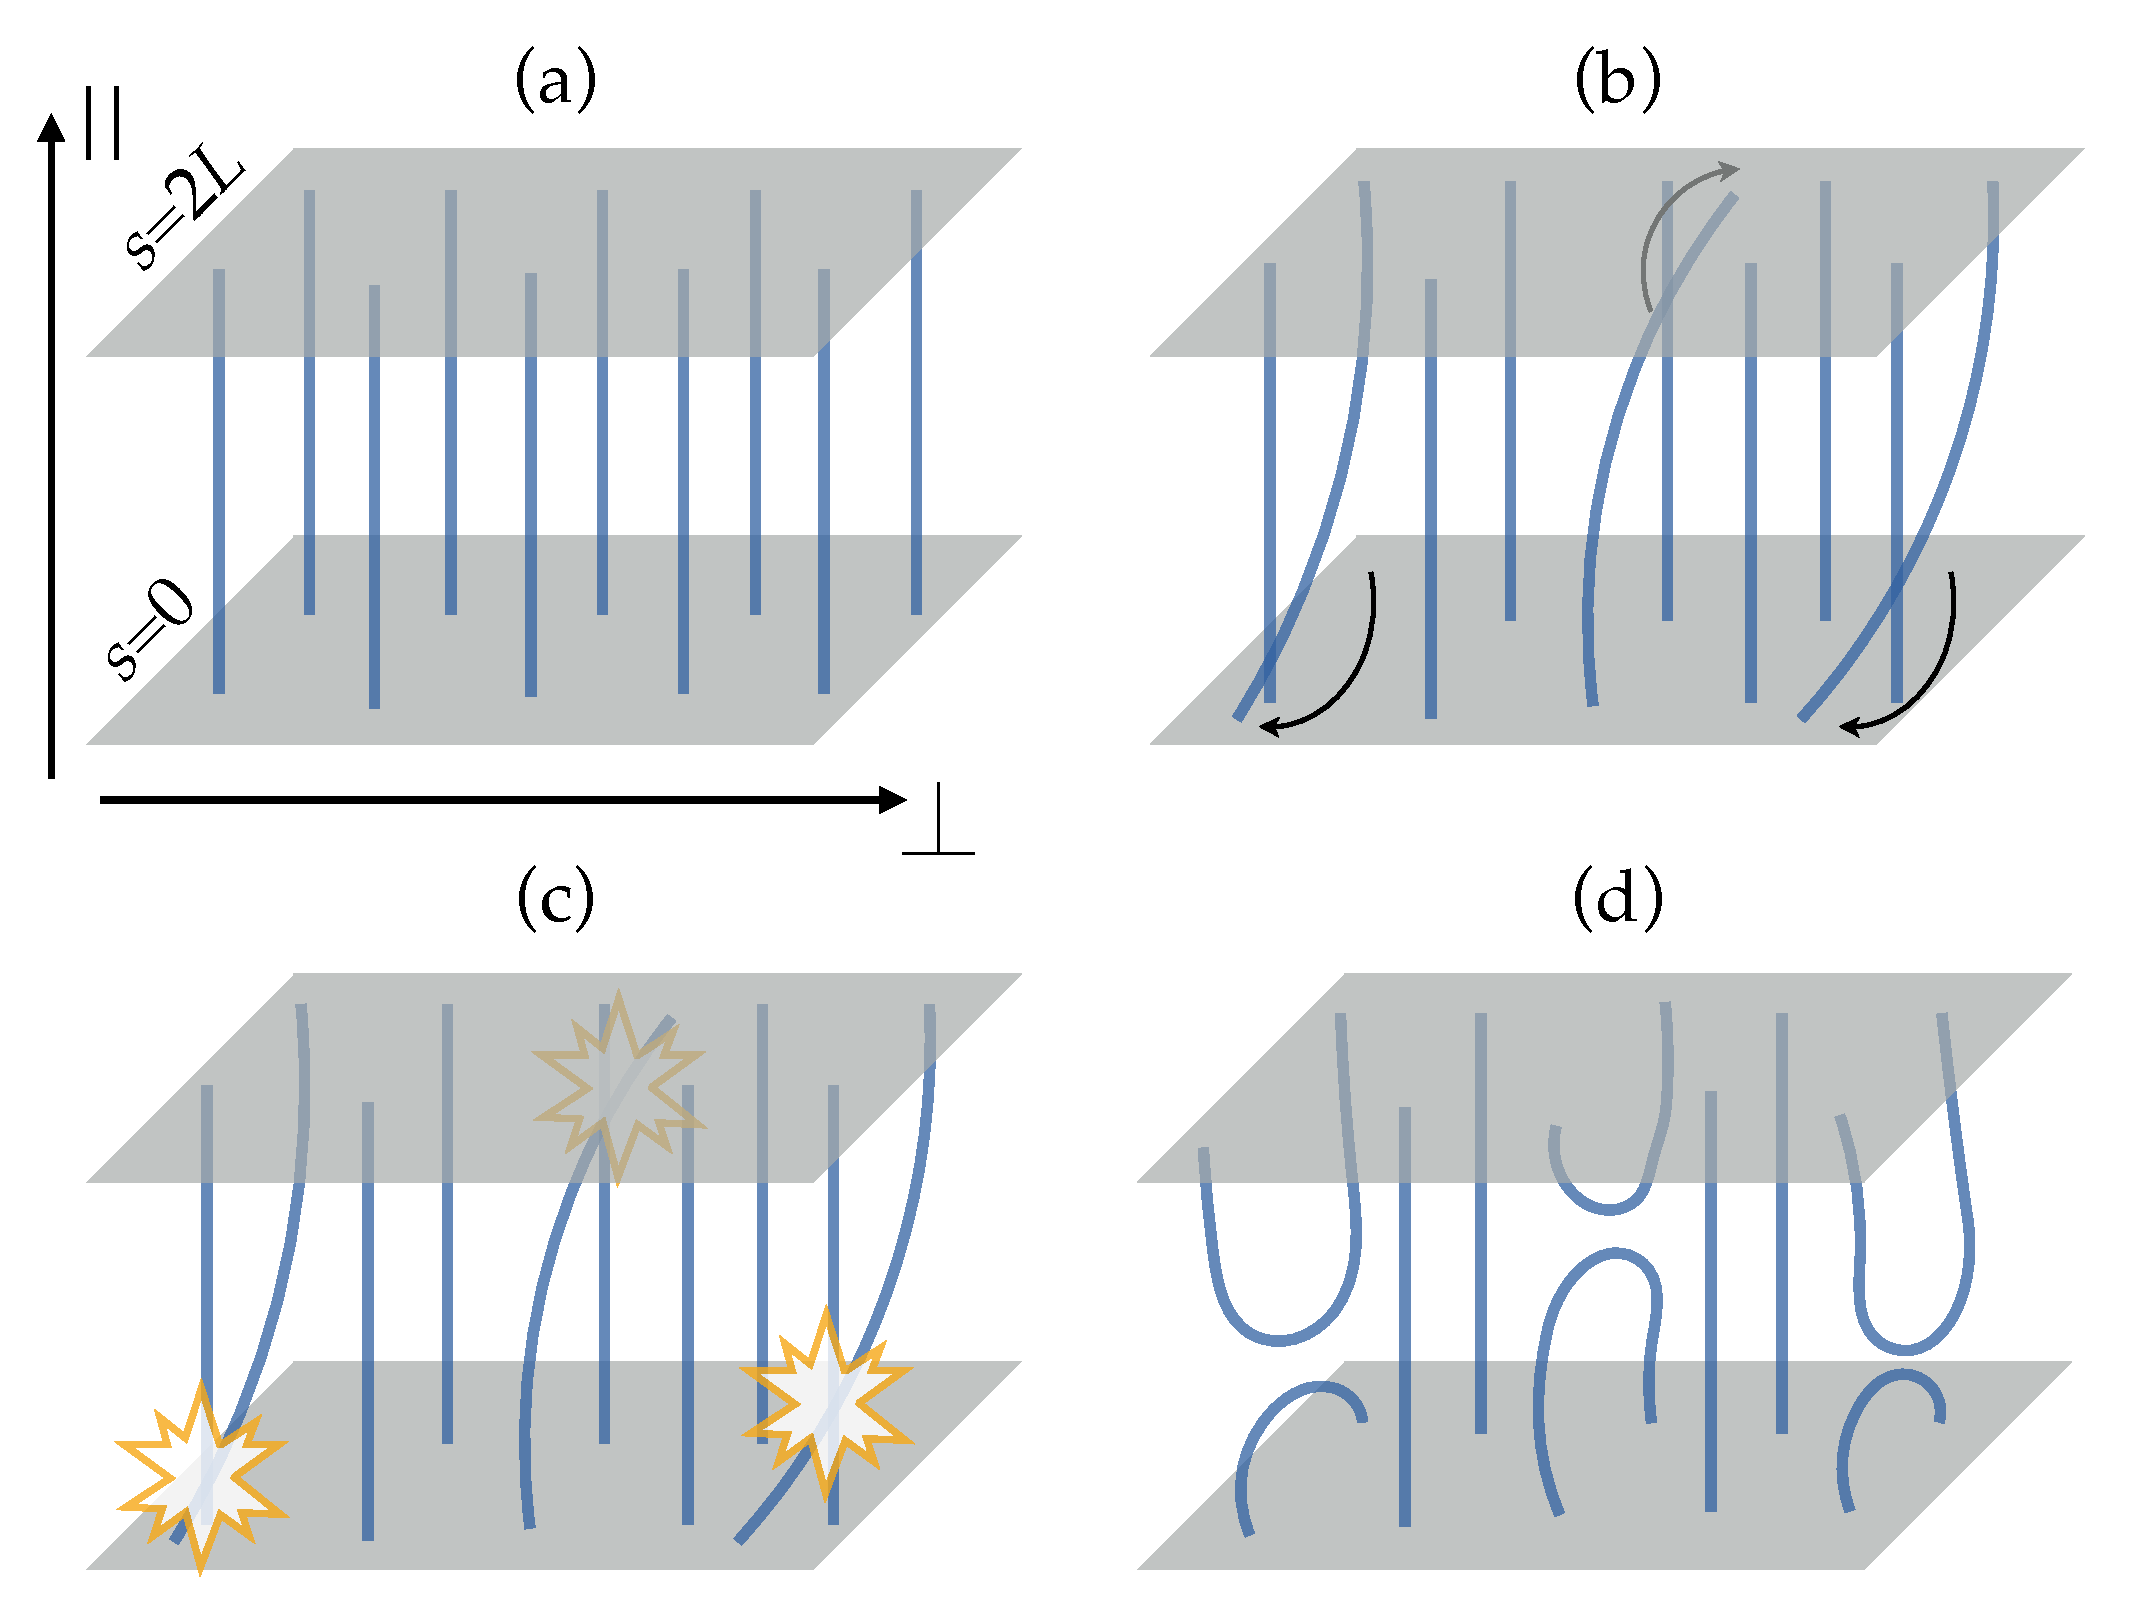
\includegraphics[width=0.75\textwidth]{chapter1/figures/nanoflare-cartoon.pdf}
    \caption{Illustration of the nanoflare heating scenario of \citet{parker_nanoflares_1988}. The flux tubes have been straightened out such that both the top and bottom gray surfaces correspond to the photosphere. Flux tubes in an initially uniform field (a) are braided when their footpoints are shuffled by the underlying convective motions of the photosphere (b). At some critical angle between the braided flux tubes, they reconnect (c) and relax back to some lower energy state (d). The axes in panel (a) indicate the directions parallel and perpendicular to the magnetic field. Adapted from Figures 5 and 7 of \citet{klimchuk_key_2015}.}
    \label{fig:nanoflare-cartoon}
\end{figure}

% spell-checker: disable %
\begin{pycode}[chapter2]
# Estimate critical angle
B_parallel = 1e2*u.G
F = 1e7 * u.erg / u.cm / u.cm / u.s
v = 0.5 * u.km / u.s
theta_c = np.arctan(4*np.pi*F.value/B_parallel.value**2/v.to(u.cm/u.s).value)
theta_c = theta_c * u.radian
\end{pycode}
% spell-checker: enable %

Following \citet{parker_nanoflares_1988}, the nanoflare energy can be estimated as follows. Consider the simplified geometry shown in \autoref{fig:nanoflare-cartoon} in which a flux tube extends from $s=0$ to $s=2L$, where both surfaces correspond to the photosphere and the flux tube has been straightened. Let the footpoint at $s=2L$ be fixed and the footpoint at $s=0$ move randomly across the surface with velocity $v$. The angle $\theta$ between the vertical and the displaced flux tube as a function of time $t$ is,
\begin{equation}
    \tan{\theta(t)} \approx \frac{vt}{2L},
\end{equation}
provided the angle is small (i.e. $\theta(t)<1$). If $B_\parallel$ is the vertical component of the field, the resulting perpendicular component can be expressed as,
\begin{equation}
    B_\perp = B_\parallel\tan{\theta(t)} \approx \frac{B_\parallel vt}{2L}.
\end{equation}
The Poynting flux associated with the work done by the footpoint motion on the field is given by,
\begin{equation}
    F = -\frac{1}{4\pi}B_\parallel\mathbf{B}_\perp\cdot\mathbf{v}_\perp = \frac{B_\parallel^2 v}{4\pi}\tan{\theta(t)} \approx \frac{B_\parallel^2 v^2 t}{4\pi(2L)}.
\end{equation}
For typical \AR{} values of $F=\SI{e7}{\erg\per\square\cm\per\second}$ \citep{withbroe_mass_1977}, $B_\parallel=\SI{100}{\gauss}$, and $v=\SI{0.5}{\km\per\second}$, $\theta\approx\py[chapter2]|f'{theta_c.to(u.degree).value:.0f}'|\si{\degree}$. Once $\theta$, the angle between $B_\perp$ and $B_\parallel$, reaches this critical value, the energy is rapidly dissipated by reconnection and the field relaxes back to its equilibrium state, destroying $B_\perp$. Note that the absence of dissipation and reconnection would result in an infinite build-up of stress in the field \citep{klimchuk_key_2015}.

Furthermore, the energy associated with each of these discontinuities in the field can be written as,
\begin{equation}
    \varepsilon = \ell^2\Delta L \frac{B_\perp^2}{8\pi},
\end{equation}
where $\ell$ is the length of each random step and $\Delta L$ is the length of winding along the neighboring flux tube. Assuming the lifetime of each step is $\approx\SI{500}{\second}$, $\ell=\SI{250}{\km}$ and $\Delta L=\ell/\tan{\theta}=\SI{e3}{\km}$. Thus, the free energy associated with the winding of the field is $\varepsilon\approx\SI{6e24}{\erg}$, in approximate agreement with observations. \citet{parker_nanoflares_1988} notes that the energy of the resulting nanoflare will, on average, be less than this value.

Much progress has been made in understanding the role of nanoflares in heating the solar corona though a definitive detection has yet to be made. Early modeling efforts by \citet{cargill_implications_1994} and \citet{cargill_nanoflare_2004} showed that nanoflares lead to a broad distribution of temperatures and can produce ``very hot'' plasma at temperatures in excess of \SI{8e6}{\kelvin}, the so-called ``smoking gun'' of nanoflare heating. While spectroscopic observations of ``warm'' \SIrange{1}{2}{\mega\kelvin} provide compelling, indirect evidence of impulsively heated plasma \citep[e.g.]{warren_constraints_2011,warren_systematic_2012,viall_evidence_2012}, a direct detection of $>\SI{8}{\mega\kelvin}$ with current instruments is not likely \citet{winebarger_defining_2012}. However, recent results from two sounding rockets, the Extreme Ultraviolet Normal Incidence Spectrograph \citep[EUNIS,][]{brosius_pervasive_2014} and the Focusing Optics X-ray Solar Imager \citep[FOXSI,][]{ishikawa_detection_2017}, provide possible detections of this very hot plasma.

Though the original nanoflare concept of \citet{parker_nanoflares_1988} was explicitly tied to reconnection, the modern definition of a nanoflare is far more general. Throughout the remainder of this thesis, I adopt the definition of \citet{klimchuk_key_2015} that a nanoflare is \textit{an impulsive energy release on a small cross-field spatial scale without regard to physical mechanism}. Nanoflares may be caused by waves or by reconnection as both have been shown to be impulsive \citep{klimchuk_solving_2006,klimchuk_key_2015}. Nanoflare events may occur frequently or infrequently on a given flux tube and their energy spectrum may be broad though it is likely to favor lower energy events \citep{hudson_solar_1991}. Rather than probing a specific physical mechanism, the work in this thesis is focused on constraining the properties of the heating, regardless of the underlying driver.

\section{Thesis Outline}\label{sec:outline}

The primary focus of this thesis is the heating of the solar corona via impulsive nanoflare heating. Understanding the energy deposition in the corona via EUV and X-ray observations is made difficult by several mitigating factors, including the optically-thin nature of the upper solar atmosphere, inadequate spectral, temporal, and spatial resolution of current observing instruments, and uncertainties in the atomic physics. A large volume of high-quality observations combined with detailed forward models are needed to adequately constrain the frequency with which energy is dissipated in the coronal plasma.

In \autoref{ch:loops} I discuss the field-aligned physics of coronal loops and detail both hydrostatic and hydrodynamic approaches to modeling the thermal structure of these loops.

In \autoref{ch:diagnostics} I outline the dominant mechanisms for producing spectral line and continuum emission in the corona. Additionally, I discuss the two primary observables used in this thesis for diagnosing the properties of the heating: the emission measure distribution and the timelag.

\autoref{ch:synthesizar} provides a detailed explanation by example of the synthesizAR forward modeling code developed for predicting optically-thin emission from an \AR{} using an ensemble of many loop models.

The next three chapters make up the primary research findings of this thesis. \autoref{ch:inferring_hot_plasma} examines signatures of nanoflare heating in the ``hot'' component of the differential emission measure distribution. In particular, I use the EBTEL model (see \autoref{sec:ebtel}) to examine the extent to which nanoflare duration, heat flux limiting, ion heating, and non-equilibrium ionization affect the observability of this very hot plasma.

In \autoref{ch:modeling-observables}, I predict the time-dependent, multi-wavelength AIA intensities from \AR{} NOAA 1158 for three different nanoflare heating frequencies using the forward modeling code described in \autoref{ch:synthesizar} combined with the EBTEL model. From these predicted intensities, I compute the emission measure slope and timelag diagnostics in each pixel of the \AR{}.

In \autoref{ch:classifying-observables}, I compute the emission measure slope and timelag from real AIA observations of \AR{} NOAA 1158. I then train a random forest classifier using the predicted diagnostics from \autoref{ch:modeling-observables} and use it to ``map'' the heating frequency across the entire \AR{} based on the classification of the observed diagnostics.

Finally, \autoref{ch:conclusions} summarizes the research findings of this thesis and suggests several topics for future work.

\section{Use of Data and Software}\label{sec:software-data}

This thesis makes use of observational data from the Helioseismic Magnetic Imager as well as the Atmospheric Imaging Assembly, both aboard the Solar Dynamics Observatory spacecraft. Data from both of these instruments are kindly made publicly available by the respective instrument teams via the Joint Science Operations \citep[JSOC,][]{couvidat_observables_2016} operated by Stanford University. All atomic data used in this work are from version 8 of the CHIANTI atomic database (see \autoref{sec:chianti}). CHIANTI is a collaborative project involving George Mason University, the University of Michigan (USA), University of Cambridge (UK), and NASA Goddard Space Flight Center (USA).

The work presented in this thesis makes use of the greater scientific Python ecosystem, including Astropy for unit-aware computation and astronomy-specific functionality \citet{the_astropy_collaboration_astropy_2018}, Dask for parallel and distributed computing \citep{dask_development_team_dask_2016}, matplotlib \citep{hunter_matplotlib_2007} and seaborn \citep{waskom_seaborn_2018} for visualization, NumPy for array computation \citep{oliphant_guide_2006}, scikit-learn for machine learning \citep{pedregosa_scikit-learn_2011}, and scipy for general purpose scientific computing \citet[e.g. interpolation, curve fitting, special functions][]{jones_scipy_2001}. This research has made use of SunPy, an open-source and free community-developed solar data analysis package written in Python \citep{sunpy_community_sunpypython_2015} and PlasmaPy, a community-developed open source core Python package for plasma physics \citep{plasmapy_community_2018_1238132}.

Additionally, this work makes use of SolarSoftware \citep[SSW][]{freeland_data_1998}, a common programming and data analysis environment for solar physics written in the proprietary Interactive Data Language (IDL).

This thesis was typeset in \LaTeX. The Python\TeX package is used to execute Python code from within the document. With the exception of \autoref{fig:nanoflare-cartoon} and \autoref{fig:heating-cooling-cycle-cartoon}, all figures are created inline in the document with Python\TeX and the texfigure Python package.

% Nomenclature
\nomenclature[a-rsun]{$R_{\solar}$}{radius of the Sun, $\approx\SI{6.957e10}{\cm}$}
\nomenclature[z-ar]{AR}{active region}
\nomenclature[z-tr]{TR}{transition region}
\nomenclature[z-mhd]{MHD}{magnetohydrodynamics}
\nomenclature[z-noaa]{NOAA}{National Oceanic and Atmospheric Administration}
\nomenclature[z-pfss]{PFSS}{potential field source surface}
\nomenclature[z-aia]{AIA}{Atmospheric Imaging Assembly}
\nomenclature[z-sdo]{SDO}{Solar Dynamics Observatory}
